\documentclass[
	11pt, 
	DIV10,
	a4paper, 
	oneside, 
	headings=normal, 
	captions=tableheading,
	final, 
	numbers=noenddot
]{scrartcl}

\usepackage{lipsum}
\usepackage{graphicx}
\usepackage{amsmath}
\usepackage{mathtools}
\usepackage{amssymb}
\usepackage{bm}
\usepackage[utf8]{inputenc}


\newcommand*\vechs[3]{
	\begin{pmatr3ix}
		#1\\
		#2\\	
		#3\\
	\end{pmatrix}
}
\newcommand*\vechb[4]{
	\begin{pmatrix}
		#1\\
		#2\\	
		#3\\
		#4\\
	\end{pmatrix}
}

%\newcommand*{\bm}{\boldsymbol}
\newcommand*\ve[1]{\vec{v}_{#1}}



\title{Example-based Plastic Deformation of Rigid Bodies}
\subtitle{\vspace{0.5cm}Seminar: Current Topics in Physically-Based Animation}
\author{Younes Müller}


\begin{document}
\maketitle
\tableofcontents
\newpage


\section{Introduction}
In modern day computer graphics gains a lot of importance. David Kriesel once stated in one of his talks that the eye is the only broad band connection to the brain \cite{dkriesel}. So the eye is the way to go to provide much detailed information to humans.
Despite the large computational effort the results need to be computed nearly in real time.\\
The field of physically based animation tightly belongs to computer graphics. A method to efficiently simulate the physical movement of objects is rigid body simulation. It assumes the objects to be unchangable. This results in very fast computations. Unfortunately deformation of objects is not initially part of the rigid body simulators.
In this seminar work I will describe and explain a method to solve this problem, described by Ben Jones, Niles Thuerey, Tamar Shinar and Adam W. Bargteil in their article "Example-based Plastic Deformation of Rigid Bodies."\cite{paper}
They developed a method, that uses deformation examples to calculate deformations on impact.
A set of example deformations are provided by an artist or a soft body simulation. Additionally to the speed of this method it gives the user the ability to control exactly, how the deformed bodies look. 
\section{Method}
\subsection{Rigid bodies}
	To simulate the translational motion of a rigid body it is sufficient to simulate the motion of the center of gravity. As the vertices stay motionless relative to the center the position of every vertex can be calculated easily from the position of the center. 
	If the motion is arbitrary it can still be represented by just a translational and a rotational movement. 
	The simulation is done by a rigid body simulator. To simulate the body it stores the following parameters:
	\begin{itemize}
		\item densitiy $\rho$ and mass $m$
		\item the moment of inertia, which is constant to each body and behaves to rotational movement, as mass behaves to translational movement.
		\item linear position $\bm{x}$ and momentum $\bm{p}$
		\item orientation $\bm \Omega$ and angular momentum $\bm L$
		\item coefficient of restitution $C_r$, which stores the ratio between elastic and non elastic collision
	\end{itemize}
	
\subsection{Skinning}
	It is far too complex to provide new positions for every single vertex. So a method named skinning is used. The mesh is rigged with bones. Every vertex is assigned to a bone. And similarly to real bones the vertices follow the movement of the bone. To prevent artifacts a vertex can not only be assinged to one bone, but to multiple bones with weighting. \\
	The bones behave a bit like real bones. For example: In a model of an arm, the bones would be placed similarly to the bones in a real arm and if the bones would be moved, the vertices would follow. A vertex at the elbow would be associated with the bone of the upper and of the lower arm, so that it follows both movements. \\
	If we have the bones $B$ have to store some more values:
\begin{itemize}
	\item undeformed mesh vertex positions: $\bm{u} \in \mathbb{R}^{N \times 3}$	
	\item skinning weights: $\bm{W} \in \mathbb{R} ^{N \times B}$
	\item the desired transformation, which consist of:
		\subitem rotation: $\bm{R} \in \mathbb{R}^{B\times 3\times 3}$
		\subitem translation: $\bm{T}\in \mathbb{R}^{B\times 3}$
\end{itemize}
The skinning weight matrix $\bm{W}$ contains a row for each vertex and a column for each bone. The Value $w_{ib}$ says how much percent of the movement of bone $b$ affects vertex $\bm x$.\\

So to get the transformed position of a single vertex we apply the weighted transformation of each bone on the vertex.
\begin{align}
\bm{x}_i =\sum_{b\in B} \bm{W}_{ib}\left(\bm{T}_b +\bm{R}_b \bm{u}_i\right)
\end{align}
As we want to use multiple example poses on every vertex we don't have one desired Transformation, but one for every pose, generated by the artist. So we extend $\bm{R}$ and $\bm{T}$ and add a matrix that contains, how much every example pose acts on every vertex:
\begin{itemize}
	\item $\bm {R}\in\mathbb{R}^{B\times E\times 3\times 3}$
	\item $\bm {T}\in \mathbb{R}^{B\times E\times 3}$
	\item $\bm{E}\in \mathbb{R}^{N \times E}$
\end{itemize}

We have to somehow consider mutliple example poses. The native approach is to use linear interpolation and weight the individual transformations with the weighting matrix $\bm{E}$.\\
We now can determine the new position of each vertex with:
\begin{align}
\bm{x}_i = \sum_{b\in B}\bm{W}_{ib}\left( \sum_{e=1}^{E} \bm{E}_{ie} \left( \bm{T}_b + \bm{R}_{be} \bm{u}_i \right) \right) 
\end{align}
With the translational part this works fairly well, however linear interpolation does not work well on rotation matrices. This is due to the fact, that a 3 dimensional rotation has 3 degrees of freedom, while a rotation matrix has 9 entries. So 6 Entries are somehow redundant and have to be bound via constraints (orhogonality and determinant is 1). So if we linearly interpolate each single entry of a roation matrix it is not guaranteed, that the resulting matrix is itself a rotation matrix. To solve this quaternion rotation is used.
\subsubsection{Quaternion rotation and QLERP}
Ken Shoemake found out that a 3 dimensional rotation can be represented by a quaternion. Quaternions are an extension of the complex numbers. They have 3 imaginary units and are based on the identity
\begin{align}
i^2=j^2=k^2=ijk=-1
\end{align}
Each Quaternion has the form: $a+ bi+cj+dk$.How exactly a quaternion can be used to rotate a vector can be read in \cite{Quat}.
Quaternion rotation has a main advantages over matrix rotation. We only have one additional entry to the 3 degress of freedom in a quaternion. So only one constraint is needed to provide a valid rotation. It turns out that a rotation quaternion has to be of length one.\\
So to interpolate between two rotations we can interpolate the corresponding rotation quaternions and normalize them. \cite{QLERP}
The formula for interpolation of the rotation quaternions $\bm q$ and $\bm p$ with the parameter $t \in[0,1]$ the following formula is used:
\begin{align}
l(t;\bm{p},\bm{q}) = \frac{(1-t)\bm{p} + t\bm{q}}{||(1-t)\bm{p} + t\bm{q}||}
\end{align}
To blend multiple rotations we now use a matrix, containing the quaternion values for each example pose $\bm{R}^{4\times E}$ and the weightings $\bm{E}^{N\times E}$. This works, because the columns of $\bm{E}$ sum up to 1.
\begin{align}
\bm{R}_i' =\text{QLERP} (\bm{E}_i,\bm{R}) = \text{normalize} \left( \sum_{e\in E} \bm{E}_{ie} \bm{R}_{e}\right)
\end{align}


\begin{figure}[tb]
	\centering
	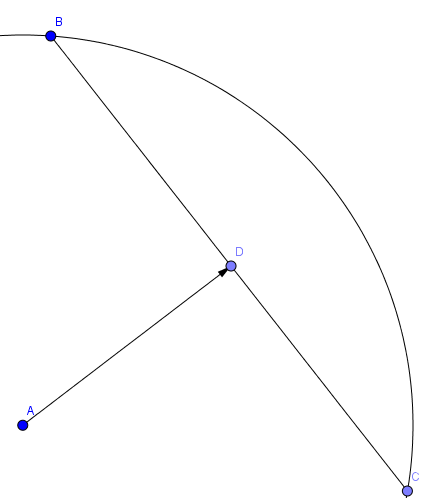
\includegraphics[width=0.3\linewidth]{images/quatrot1} 
	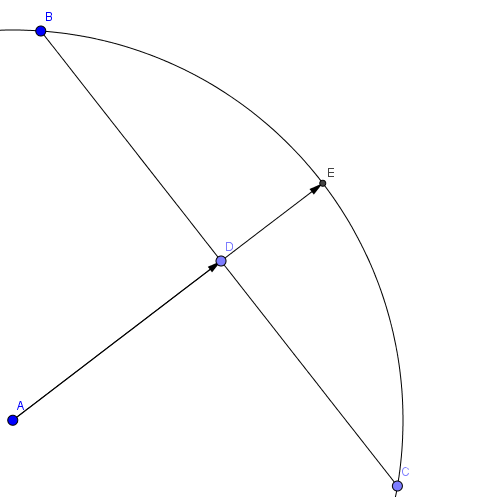
\includegraphics[width=0.33\linewidth]{images/quatrot2} 
	\caption{\label{fig:image} On the left: Idea, how linear interpolation between rotation matrices looks. If linear interpolation between two points on a circle is used, the resulting points do not lie on the circle. On the right: Interpolating with quaternions. The result can be easily mapped onto the sphere by normalizing the quaternion.
	}
\end{figure}



\marginpar{Ist das hier okay, dass ich die Notation der Matritzen missbrauche? Der erste Parameter der Rotationatrix ist ja eigentlich, welches Element eines Quaternions verwendet wird, aber aus der Notation wird denke ich klar, dass statdessen der einem Beispiel zugeordnete quaternion gemeint ist.}

\subsection{Recap Skinning}
Now we have a method to deform meshes with the help of bones and to blend in given example poses.
The input consists the constant data:
\begin{itemize}
\item The Vertex positions in undeformed state: $\bm u\in\mathbb{R}^{N\times 3}$
\item The weighting of each bone for the vertcies: $\bm W\in\mathbb{R} ^{N \times B}$
\item The transformation for each example pose, consiting of
	\subitem The rotational part $\bm R\in\mathbb{R}^{B\times 4\times  E}$
	\subitem The translational part $\bm T\in\mathbb{R}^{B \times 3\times E}$
\end{itemize}
and the changing data:
\begin{itemize}
	\item example Weights $\bm{E}\in\mathbb{R}^{N\times E}$
\end{itemize}
Let $\text{rotate} (\bm{q},\bm{x})$ be the function that rotates the position $\bm{x}$ by the quaternion $\bm{q}$.
The skinned mesh vertex positions $\bm{x} \in \mathbb{R}^{N\times 3}$ can now be calculated by:
\begin{align}
\bm{x}_i = \sum_{b\in B} \bm{W}_{ib}\left(\sum_{e=1}^{E}\bm{E}_{ie}\bm{T}_{be} + \text{rotate}(\text{QLERP}(\bm{E}_i,\bm{R}_b),\bm{u}_i)\right)
\end{align}

% !TeX encoding = UTF-8
\subsection{Calculate example weighting}
When two objects collide, the rigid body simulator passes the vertex $\bm{x}_i$, where the collision occurred and the impulse $\bm{j}_i$.
The goal is now to calculate a 	useful configuration of the example weights, that matches the impact. As example poses are used, not every deformation is possible. So we first calculate an ideal deformation for the vertex being hit. Then we solve a minimization problem, trying to get good example weightings, so that the distance between the ideal deformation and the skinned position of the vertex is minimal. Afterwards we propagate this to the vertices around.
\subsubsection{Projection}
The formula for the ideal deformation is given by:
\begin{align}
\bm{\Delta x}_i = \frac{\Delta t}{m} \max(||\bm{j}_i|| - \beta, 0) \frac{\bm j_i}{||\bm j_i||}
\end{align}
It extends the usual formula for the deformation $\bm{\Delta x}_i = \frac{\Delta t}{m} \bm j_i$ with the user adjustable threshold $\beta$, on how strong the impact has to be at minimum to be registered. This prevents deformation on resting contact.
The term $\Delta t$ is the size of a timestep and $m$ is the mass of the object.
We now construct the Jacobian matrix $\bm J$ by
\begin{align}
\bm J_i = \frac{\partial\bm x_i}{\partial \bm E_{ie}} \in \mathbb{R}^{3\times E}
\end{align}
It contains the change in vertex position depending on a change in the example weighting.
So given a change of position $\Delta x$, in the example space we can compute the change of example weightings by:
\begin{align}
\bm{\Delta e}_i = \bm J_i^T \bm{\Delta x}_i
\end{align}
This formula however requires the change to be in the space of possible changes, that can be achieved by the examples. To get a good $\bm{\Delta e}$ we have to minimmize the following problem:
\begin{align}
\bm{\Delta e} = \min_{\bm{\Delta \hat e}}||(\bm x_i (\bm e + \bm{\Delta \hat e}) -\bm x_i (\bm e )) - \bm{\Delta x}_i ||^2
\end{align}
A method to solve minimization problems is the method of steepest descent. The direction of the gradients, which points in the direction of steepest ascent on every point on the (hyper-)plane is used to iteratively go in the direction of the steepest descent to search a lokal minimum.
As we do not opt for physical accuracy it is sufficient to go one step. As initial value $\bm{\Delta e} = 0$ is used. The gradients can be calculated by transposing the Jacobi matrix:
\begin{align}
\frac{\bm J_i^T \bm{\Delta x}_i}{||\bm J_i^T \bm{\Delta x}_i||}
\end{align}
is the direction of the gradient on $\Delta x$

The stepwidth of the step is chosen, so that it is dependent on the impact and user controllable.
The approximated change in Example weightings is calculated by:
\begin{align}
\bm{\Delta e}_i = \alpha ||\bm{\Delta x}|| \frac{\bm J_i^T \bm{\Delta x}_i}{||\bm J_i^T \bm{\Delta x}_i||}
\end{align}

\subsection{Propagation}
If we would apply the change in example weights only on the vertices, that were hit, the result would look bumpy. So the change in example weights is propagated to nearby vertices. As distance measure, the approximated geodesic distance via a few Dijkstra iteration is used. The change of Example weights for every vertex is saved in the Matrix $\bm{\Delta E}$. To propagate the change we modify each column by:
\begin{align}
\bm{\Delta E}_j \;+\!\!= \phi\left(\frac{||\bm x_j - \bm x_i||}{\gamma}\right) \bm{\Delta e}_i\\
\phi(x) =
\begin{cases}
	2x^3 - 3x^2 + 1 & : x< 1\\
	0               & : otherwise	
\end{cases}
\end{align}
This assures that the vertecies within a user determined distance $\gamma$ of the impacted vertexare also affected.
\subsection{Application}
To let the impact look more natural, the deforming does not happen instantaneously, but over time.
The Matrix $\bm{\Delta E}$ contains the change in example weighting that still has to be applicated. In every timestep the current example weighting $\bm E$ and $\bm{\Delta E}$ are updated via:
\begin{align}
\bm E \;+\!\!= (1-\lambda)\bm{\Delta E} \\
\bm {\Delta E} \;*\!\!= \lambda
\end{align}
where $\lambda$ is a user given parameter. For $t\rightarrow\infty$ the whole change is applicated.
\subsection{Restitution Modifiaction}
As a deformation consumes energy it is necessary to show this in the movement of the object. With the deformation the nonelastic part of the collision increases. The ration between the elastic and non-elastic part, the coefficient of restitution is modified by:
\begin{align}
C_r := \min(C_r^*, C_r + \mu \Delta t, \exp(-\nu||\bm{\Delta E}||_f)C_r^*)
\end{align}
where $C_r^*$ is the coefficient that is initially used by the rigid body simulator and $\mu$ and $\mu$ are user given.



\subsection{Userparameters}
The following parameters are adjustable by the user and determine:
\begin{itemize}
	\item $\alpha$: how much the impact deforms the bodies
	\item $\beta$: how strong the impact has to be to be noticed
	\item $\gamma$: how far the deformation is propagated
	\item $\lambda$: how long the deformation should take
	\item $\mu$ and $\nu$: how elastic the collision is modified
\end{itemize}
\subsection{Fracture}
Fracturing of the mesh is supported. It is achieved by splitting the mesh in individual parts. The parts are hold together by constraints. If a force exceeds a threshold the contraints are removed and the model is fractured.
\section{Discussion}
\subsection{Performance}
Using the method to simulate deformation adds a avarage of 42\% to 59\% every timestep in the tests. It is significantly slower than regular rigid body simulation, because the meshes are not convex and collision detection is faster on convex meshes.
\subsection{Future Work}
A possible improvement would be automated rigging. Then example poses can be provided by soft body simulators and integrated into the system.\\
Implementing an application for modeling the objects or integrating a plugin for a given application would give the possitility to modify parameters with brushes individually for the vertices.



\bibliographystyle{alpha}
\bibliography{references}

\end{document}          
